\begin{figure}[H]
  \centering
  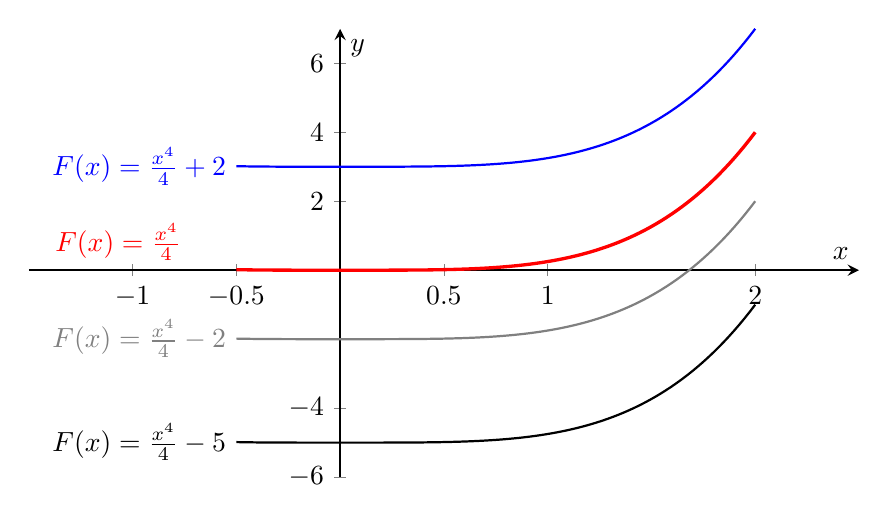
\begin{tikzpicture}
    \begin{axis}[
      width = \textwidth,
      height=\axisdefaultheight,
      xmin = -1.5, xmax = 2.5, ymin = -6, ymax = 7,
      axis lines = middle,
      xlabel = $x$,
      ylabel = $y$,
      samples = 100,
      thick,
      xtick = {-1, -.5, .5, 1, 2},
      ytick = {-6, -4, 2, 4, 6}
      ]
      \addplot[very thick, domain=-.5:2, color=red]{x^4/4} node[xshift=-16pt, yshift=10pt, left, pos=0]{$F(x) = \frac{x^{4}}{4}$};
      \addplot[domain=-.5:2, color=blue]{x^4/4 + 3} node[left, pos=0]{$F(x) = \frac{x^{4}}{4} + 2$};
      \addplot[domain=-.5:2, color=gray]{x^4/4 - 2} node[left,pos=0]{$F(x) = \frac{x^{4}}{4} - 2$};
      \addplot[domain=-.5:2, color=black]{x^4/4 - 5} node[left,pos=0]{$F(x) = \frac{x^{4}}{4} - 5$};
    \end{axis}
  \end{tikzpicture}
  \caption{Графики некоторых первообразных функции $x^3$}
  \label{tikzplot:Antiderivative_x_Cubed}
\end{figure}
